% Chapter Template

\chapter{Experimental Results} % Main chapter title

\label{chp:results} % Change X to a consecutive number; for referencing this chapter elsewhere, use~\ref{ChapterX}
In this chapter proposed methodologies are evaluated and compared with the related work.

All models are Trained using QaTa-Cov-19~\cite{ahishali2021advance} dataset using NVIDIA Tesla P-100 GPU and programmed using PyTorch.
\section{QaTa-COV19 Dataset}
\begin{center}
\begin{figure}[htbp]
\centerline{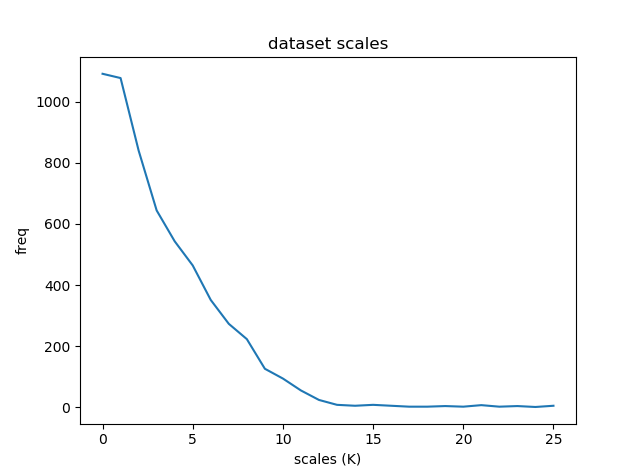
\includegraphics[height=60mm,width=9cm]{ScaleDist.png}}
\caption{Pneumonia Scales of QaTa-COV19-v1, Y-axis represents the frequency, number of occurrences, of pneumonia with a particular area}
\label{pdist}
\end{figure}
\end{center}
QaTa-COV19 is a benchmark dataset for COVID-19 detection and Segmentation from CXR images. All models used for comparison are trained using QaTa-COV19-v1. Qata-COV19-v1 consists of 4603 COVID-19 CXRs and $120,013$ control group CXRs. A balanced number of samples for the two classes is used, namely 4603 CXR images for each class to train the models. Pneumonia Scales of QaTa-COV19-v1 do not exhibit a uniform distribution. The scale of the Pneumonia can be defined as the number, area, of 8-neighbor-connected pixels labeled as COVID-19 pneumonia. QaTa-COV19-v1 provides a binary mask of 2951 COVID-19 CXR images which can be used for approximating the distribution of scales across the dataset. Fig.~\ref{pdist} illustrates the statistical distribution of QaTa-COV19 scales. The non-uniform distribution of the scales allows the CNN models to only recognize the small scales and not the large scales.

\section{Evaluation of the Methodology I}

Experiments are conducted on a Lenovo Z50-70 with Intel CORE i7-4510U CPU 2.00 GHz, 8GB RAM, NVIDIA GeForce 840M GPU; and with Python and PyTorch library.

\subsection{Details of the Proposed Architecture}
The Proposed architecture is composed of Convbase and Densebase. Convbase is composed of a $6$ feature extraction modules \textit{(FX)} preceded by batch normalization layer. Each FX module can be considered a sub-sequential model consisting of an RSB layer followed by Batch Normalization, Max-pooling, and LeakyReLU activation function. The Densebase is two fully connected layers that classify the Convbase output.


\subsection{Hyperparameter Specification}
All input chest X-ray images are resized to be $200\times 200$ . After resizing the input images, these images are fed the Convbase model part which consists of 6 layers of residual separated block. Each residual separated block is followed with batch normalization and LeakyReLU~\cite{he2015delving} as an activation function. The output depth of each residual separated block is 4$\times$16, 4$\times$32, 4$\times$64, 4$\times$64, 4$\times$64, and 4$\times$16, respectively. The output of the Convbase model part is a 1D feature vector of 576 in length. The densebase model part consists of two hidden layers. Each layer has a size of 64 and the output layer of size 2. Each layer of Densebase layers is fully connected to its previous layer. The activation function used in the densebase model part is LeakyReLU. Table~\ref{lyrSpec} summarizes the architecture hyperparameters.

\begin{table}[htbp]
\caption{The proposed architecture hyperparameters}
\begin{center}

\begin{tabular}{|l|c|c|}
\hline
\textbf{Layer Number} & \textbf{Layer Size} & \textbf{Activation Function} \\
\hline
\hline
RSBLayer1 & 4 $\times$ 16 & LeakyReLU\\
\hline
RSBLayer2 & 4 $\times$ 23 & LeakyReLU\\
\hline
RSBLayer3 & 4 $\times$ 64 & LeakyReLU\\
\hline
RSBLayer4 & 4 $\times$ 64 & LeakyReLU\\
\hline
RSBLayer5 & 4 $\times$ 64 & LeakyReLU\\
\hline
RSBLayer6 & 4 $\times$ 16 & LeakyReLU\\
\hline
\multicolumn{3}{|c|}{\textit{Flatten The Feature maps to 1D 576 feature  vector}}\\
\cline{1-3}
LinearLayer1 & 64 & LeakyReLU\\
\hline
LinearLayer2 & 64 & LeakyReLU\\
\hline
LinearLayer3 & 2 & Softmax\\
\hline
\end{tabular}
\label{lyrSpec}
\end{center}
\end{table}

\subsection{Network Training}
The proposed CNN model is trained for 22 epochs. Adaptive Moment Estimation (Adam) optimizer~\cite{kingma2014adam} is a popular optimization technique for training deep networks. Adam optimizer is used during the training phase of the proposed CNN model. Both batch size and Adam optimizer learning rate are changed during the training phase if the training loss stops decreasing. Table~\ref{tabTrparam} summarizes the parameter values used in the training phase of the proposed CNN model. Fig.~\ref{fig5}(a) shows the progress for training and validation loss across each epoch. The difference between the training loss and validation loss through epochs shows that we did not memorize the dataset.
\begin{table}[htbp]
\caption{The change of batch size and learning rate through the Training process}
\begin{center}

\begin{tabular}{|l|c|c|}
\hline
\textbf{Epoch Number} & \textbf{Batch Size} & \textbf{Learning Rate} \\
\hline
\hline
From 0 to 6 & 128 & 1e-3\\
\hline
From 7 to 12 & 256 & 1e-3\\
\hline
From 13 to 21 & 256 & 1e-4\\
\hline
 
\end{tabular}
\label{tabTrparam}
\end{center}
\end{table}



\subsection{Model Evaluation}

To assess the efficiency of the proposed method,  the proposed method is compared to recent state-of-the-art methods for detecting Covid-19 cases. Experiments are conducted with the same dataset and the corresponding hyperparameter of each work. All the methods depend on CNN. The comparison is performed using precision, sensitivity, F1-score, and accuracy~\cite{hossin2015review}. In addition, the number of parameters used in the training phase is a very important comparison factor. Table~\ref{modelperf} depicts the comparison between state-of-the-art methods and the proposed method. As shown in the comparison, the proposed method outperforms other methods achieving the maximum accuracy and the lowest parameter count. 



\begin{table}[htbp]
\caption{ A performance comparison between the proposed method and state-of-the-art models.}
\begin{center}
\begin{tabular}{|l|c|c|c|c|c|}
\hline
\textbf{Method} & \textbf{PC} & \textbf{P(\%)}& \textbf{S(\%)}& \textbf{F1(\%)}& \textbf{A(\%)} \\
\hline
\hline
Proposed Method & 0.15M & 100.00 & 100.00 & 100.00 &100.00\\
\hline
ResNet-34~\cite{nayak2021application} & 21.8M & 96.77& 100.00 & 98.36 &98.33  \\
\hline
ACoS Phase I~\cite{chandra2021coronavirus}& - & 98.266 & 96.512 & 98.551 & 98.062 \\
\hline
ResNet-50~\cite{nayak2021application}& 25.6M& 95.24& 100.00& 97.56& 97.50 \\
\hline
GoogleNet~\cite{nayak2021application}& 5M &96.67& 96.67& 96.67& 96.67 \\
\hline
VGG-16~\cite{nayak2021application}& 138M& 95.08 & 96.67 & 95.87 &95.83\\
\hline
AlexNet~\cite{nayak2021application}& 60M& 96.72 &98.33 & 97.52& 97.50 \\
\hline
MobileNet-V2~\cite{nayak2021application} & 3.4M &98.24& 93.33& 95.73 & 95.83 \\
\hline
Inception-V3~\cite{nayak2021application}& 24M &96.36& 88.33 & 92.17& 92.50\\
\hline
SqueezeNet~\cite{nayak2021application}& 1.25M &98.27 &95.00& 96.61& 96.67 \\
\hline
\multicolumn{6}{l}{\textit{ PC is Parameter count, P is precision, S is sensitivity }}\\
\multicolumn{6}{l}{\textit{  F1 is F1-score, and A is accuracy }}\\
\hline
\end{tabular}
\label{modelperf}
\end{center}
\end{table}


\begin{figure}
\begin{center}
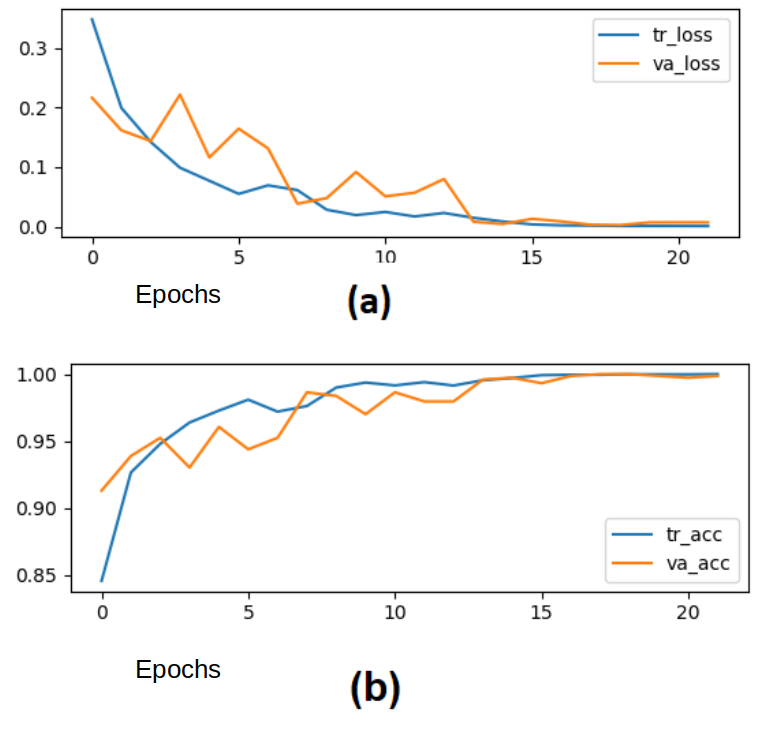
\includegraphics[height=90mm,width=8.0cm]{Figures/fig6.png}
\caption{(a) The training loss and the validation loss of each epoch and (b) The training accuracy and the validation accuracy of each epoch.}\label{fig5}\end{center}\end{figure}



\section{Evaluation of the Methodology II}
Methodology II is evaluated and compared against strong baselines and related works. 

\subsection{Baseline Networks}
Different architectures are trained to validate the effectiveness of the proposed method. 
\subsubsection{Spatial Pyramid Pooling (SPP-net) Based model}
Four variants of SPP-net\cite{he2015spatial} is trained. All $4$ variants have the same architecture but different SPP-layer. These variants of SPP-layer are as follows:
\begin{itemize}
  \item full pyramid SPP of 8-levels using average-pooling as an aggregation function
  \item full SPP pyramid of 8-levels using max-pooling as an aggregation function
  \item single level SPP with 10-bins using average-pooling as an aggregation function
  \item single level SPP with 10-bins using max-pooling as an aggregation function
\end{itemize}
  A Fixed Architecture is used for all SPP variant models with the same design principles of the proposed architecture. These architectures are the same as the proposed architecture but DSWASPP is replaced by DC6 and SPP-1 layer is replaced with the corresponding SPP layer. DC6 is defined as six convolutional layers Densely connected. For SPP-net variants training a multiscale augmentation is added to the proposed augmentation process. Multiscale augmentation is done by randomly sampling different $5$ scales typically $\{320, 320\pm25, 320\pm50 \}$.
\subsubsection{Switchable Atrous Spatial Pyramid Pooling (SASPP-net) Based models} 
\begin{center}
\begin{figure*}[htbp]
\centerline{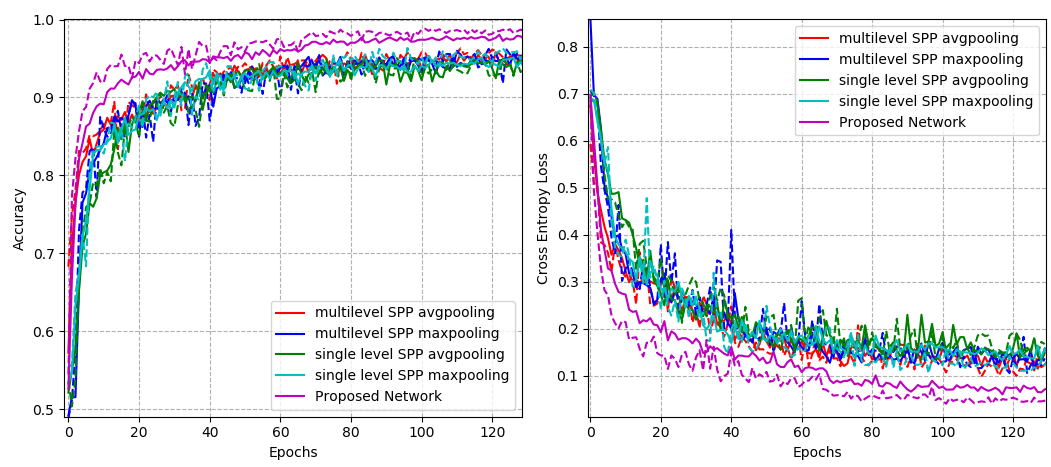
\includegraphics[height=63mm,width=15cm]{SPP-netsTraining.PNG}}
\caption{Training profiles of both SPP-net variants and the proposed network. For the same color solid line represents training statistics while the dashed line represents the validation statistics for the corresponding model. \textbf{left:} is the training accuracy. \textbf{Right:} is the training loss.}
\label{SPP-train}
\end{figure*}
\end{center}

Another Baseline is introduced for comparison which is exactly as same as the proposed network but with a different Attention module structure and does not include a bottleneck within ASPP. This architecture is referred to as Switchable Atrous Spatial Pyramid Pooling (SASPP-net). The attention module structure is $Softmax(FC(GAP(X)))$ where: \textit{$X$: is the input feature map}, \textit{$GAP$: is a global average pooling}, \textit{$FC$: is fully Connected layer performs a non-linear projection to ${\rm I\!R}^{4}$ 4 values for the three scales and the input feature map}.\\

\begin{table}[htbp]
\caption{Baselines and their total number of parameters}
\begin{center}
\begin{tabular}{|c|c|c|}
\hline
\textbf{Model}&\multicolumn{2}{|c|}{\textbf{Baseline CNN Architectures}} \\
\cline{2-3} 
\textbf{Type} & \textbf{\textit{Variant}}& \textbf{\textit{Param. Count}} \\
\hline
  & ML Average pooling & $14,916,420$   \\
\cline{2-3} 
SPP & ML max pooling & $14,916,420$   \\
\cline{2-3} 
  & SL Average pooling & $14,490,436$   \\
\cline{2-3} 
  & SL max pooling & $14,490,436$ \\
\hline
\multicolumn{2}{|c|}{SASPP} & $13,031,841$\\
\hline
\multicolumn{3}{l}{ \textbf{ML}: Multilevel, \textbf{SL}: Single level}
\end{tabular}
\label{Basarch}
\end{center}
\end{table}
Table~\ref{Basarch} summarizes the baseline models and the Corresponding parameter count.
\subsection{Models Training}
The proposed architecture and baseline architecture are trained with the same hyperparameters. The dataset is split into $0.6$, $0.2$, and $0.2$ for training, validation, and testing, respectively. For training a Cross Entropy Loss is used. All models trained with ADAM~\cite{kingma2014adam} optimizer with learning rate start by $10^{-3}$ and reduced every time validation loss plateau by multiplying by $10^{-1}$. A Max Norm Constraint is used to clip the gradient value to the norm of $1$~\cite{krizhevsky2012imagenet}. A batch size of $128$ is used to calculate the gradient.
\subsection{Reducing the overfitting}
Overfitting is a critical problem for training large networks~\cite{krizhevsky2012imagenet}. The proposed work has reduced the overfitting by using:
\begin{itemize}
\item Using Dropout with retrain probability of $0.5$~\cite{srivastava2014dropout}.
\item Using BatchNorm adds noise due to randomization introduced when constructing the minibatch~\cite{ioffe2015batch}.
\item Using max norm constraint~\cite{krizhevsky2012imagenet}.
\item Deep and thin architectures by design have an implicit regularization effect~\cite{he2016deep}. 
\item Augmentation process i.e.) Texture augmentation~\cite{krizhevsky2012imagenet}. 
\item The use of small kernel size~\cite{simonyan2014very}.
\item Bottleneck in SWASPP module and the attention module.
\end{itemize}
During training no overfitting effects are observed.
\subsection{Comparison with baselines}
The proposed network is compared with the vanilla SPP-based Architecture and ASPP architecture.
\subsubsection{Comparing with SPP-nets}
Fig.~\ref{SPP-train} illustrates both training loss and training and validation accuracies and losses. Table~\ref{blaccom} illustrates the testing accuracy for comparison between the SPP-nets baseline and the proposed architecture.
\begin{table}[htbp]
\caption{Comparison between Proposed network and baseline SPP architectures }
\begin{center}
\begin{tabular}{|c|c|}
\hline
\textbf{Model Name}& Accuracy \\
\hline
 SPP ML Average pooling & $0.958$   \\
\hline
SPP ML max pooling & $0.950$   \\
\hline
  SPP SL Average pooling & $0.927$   \\
\hline
  SPP SL max pooling & $0.957$ \\
\hline
Proposed Network & $0.987$\\
\hline
\multicolumn{2}{l}{ \textbf{ML}: Multilevel, \textbf{SL}: Single level}
\end{tabular}
\label{blaccom}
\end{center}
\end{table}
\subsubsection{Comparing with SASPP}
Fig.~\ref{saspp} illustrates the training and validation loss of training a SASPP baseline architecture. As shown in Fig.~\ref{saspp} SASPP is unable to generalize and start overfitting the training set. This comparison empirically shows the importance of the bottleneck introduced in the proposed architecture.

\begin{center}
\begin{figure}[htbp]
\centerline{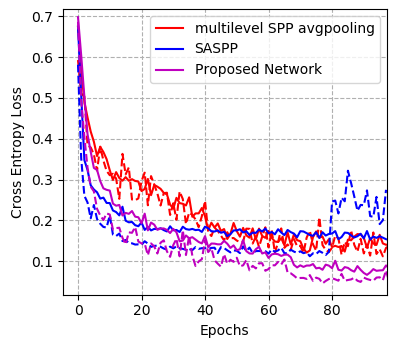
\includegraphics[height=55mm,width=8cm]{saspp.PNG}}
\caption{SASPP baseline architecture loss during both training, solid line, and validation, bashed line, compared with Proposed network and best performing SPP architecture.}
\label{saspp}
\end{figure}
\end{center}

\subsection{Comparing with the related works}
To fairly compare with the related works proposed work is further trained. Fig.~\ref{ploss} shows the training and validation loss of the proposed network. Fig.~\ref{pacc} shows the of the training and validation accuracy. 
\begin{center}
\begin{figure}[htbp]
\centerline{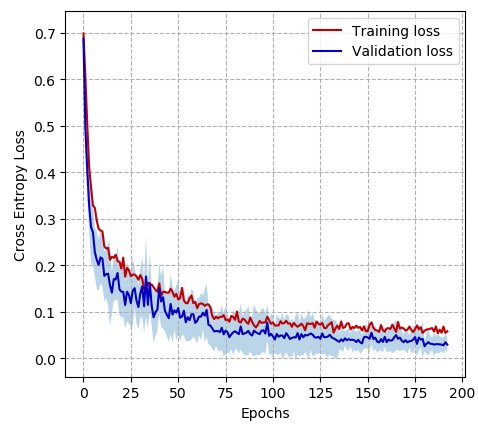
\includegraphics[height=55mm,width=8cm]{PLOSS.PNG}}
\caption{Cross entropy loss of the proposed architecture.}
\label{ploss}
\end{figure}
\end{center}
\begin{center}
\begin{figure}[htbp]
\centerline{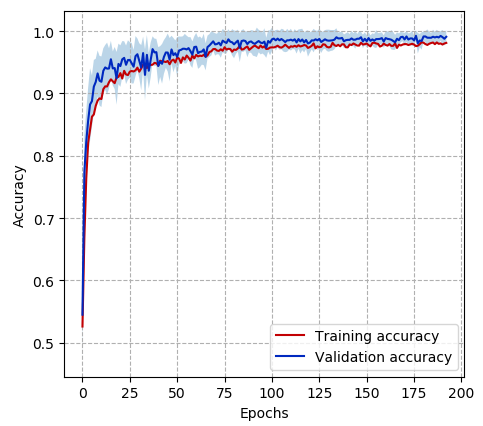
\includegraphics[height=55mm,width=8cm]{PACC.PNG}}
\caption{Training and validation accuracy of the proposed architecture.}
\label{pacc}
\end{figure}
\end{center}
The proposed Network has a sensitivity, recall, and precision of $0.994$ and $0.991$ respectively on the validation set. Precision can be improved by investigating the precision-recall trade-off. Fig.~\ref{prt} shows the trade-off between precision and recall for different thresholds. A threshold of $0.618$ is used to improve the precision resulting in a sensitivity, recall, of $0.9903$ and precision of $0.9956$.
Comparison metrics are defined as follows:
\begin{itemize}
\item \textit{Accuracy}: is the ratio of correctly classified samples to the total number of samples
\item \textit{Sensitivity}: is the ratio of correctly classified Covid-19 samples to the total number of actual Covid-19 samples 
\item \textit{Precision}: is the ratio of correctly, according to the ground-truth labels, classified Covid-19 samples to the total number of samples classified as Covid-19.
\item \textit{Specificity}: is the ratio of correctly, according to the ground-truth labels, classified non-COVID-19 to the total number of non-COVID-19.
\item \textit{F1-score}: is the harmonic mean of both Sensitivity and Precision.
\begin{center}  
 $F_{1}=\frac{2\times\text{Precision} \times \text{Sensitivity}}{\text{Precision} + \text{Sensitivity}}$
\end{center}
\item \textit{Param. Count}: is the total number of the trainable parameters.
\end{itemize}


\begin{table*}[!p!t]
\caption{Comparison between Proposed network and Related works }
\begin{center}
\resizebox{\textwidth}{!}{\begin{tabular}{|c|c|c|c|c|c|c|}
\hline
\textbf{Model Name}& \textbf{Accuracy} & \textbf{Sensitivity} &\textbf{ Precision} & \textbf{Specificity} & \textbf{F1-score} & \textbf{Param. Count}\\
\hline
\hline
Proposed & 0.99294 & \textbf{0.9903} & \textbf{0.9956} & 0.9956 & \textbf{0.9929} & \textbf{5,040,571}\\
\hline
SRC-Dalm\cite{ar} & 0.985 & 0.886 & - & 0.993 & - & -\\
\hline 
SRC-Hom\cite{ar} & 0.977 & 0.921 & - & 0.982 & - & - \\
\hline
CRC-light\cite{ar} & 0.973 & 0.955 & - & 0.974 & - &- \\
\hline
DenseNet121*\cite{ar} & 0.992 & 0.9714 & - & 0.9949 & - & 6,955,906  \\
\hline
Inception-v3\cite{ar} & 0.993 & 0.954 & - & 0.998 & - & 21,772,450  \\
\hline
Modified MobileNetV2~\cite{akt}  & 0.98 & 0.98 & 0.97 & - & 0.97 & -\\
\hline
ReCovNet-v2\cite{dag} & 0.99726 & 0.98571 & 0.94262 & 0.9977 & 0.96369 &- \\
\hline
ReCovNet-v1\cite{dag} & 0.99824 & 0.9781 & 0.97438 & 0.99901 & 0.97624 & -\\
\hline
DenseNet-121\cite{dag}  & \textbf{0.9988} & 0.97429 & 0.9932 & \textbf{0.99974} & 0.98365 & 6,955,906 \\
\hline
\end{tabular}}
\end{center}
\label{rwcom}
\end{table*}


\begin{center}
\begin{figure}[htbp]
\centerline{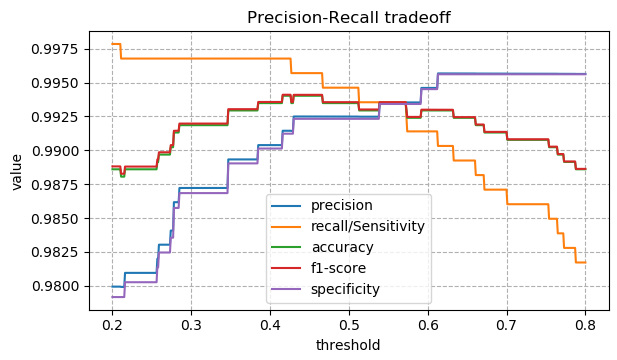
\includegraphics[height=55mm,width=8cm]{PresRecuTradff.PNG}}
\caption{precision-recall trade-off of the proposed network.}
\label{prt}
\end{figure}
\end{center}

Table~\ref{rwcom} summarizes the comparison between the recent related works and the proposed architecture. The proposed architecture outperforms these works in many metrics. As their training and testing do not depend on a balanced number of samples, accuracy, and specificity are not good metrics for evaluation. 


\section{Summary}
% This chapter illustrates the superior performance of the proposed works I and II. Experimental results of proposed work I show the effectiveness of spatial separable kernels and residual connection for detecting COVID-19. The proposed architecture I uses batch normalization to maintain the network stability during the training process. During the training process, the hyperparameters (such as batch size and learning rate) are determined dynamically. Proposed architecture I outperformed previous works for binary classification of chest X-ray images to normal or COVID-19 cases. The proposed architecture has a very low parameter count (150K trainable parameter) compared to previous work. The proposed architecture I achieved a performance of 100\% for accuracy, sensitivity, precision, and F1-score. Proposed work I does not take care of the fact that CNN is a scale variant model while proposed work II does. Better quantitative results for CXR COVID-19 classification can be obtained with multiscale training approaches. Proposed work II internally produces multiscale feature maps using Atrous Spatial pyramid pooling. These multiscale feature maps are fused using an attention module. To learn a compact representation a bottleneck dimension is introduced in both the multiscale feature extractor module and the attention module. Proposed work II outperformed current state-of-the-art architecture with a lower parameter number. The proposed method has recorded a $0.9929$ for $F1-score$.


This chapter illustrates the superior performance of the proposed work I and II. In addition to the superior performance of the proposed works I and II, the chapter also provides a detailed analysis of the experimental results. The evaluation of proposed work I demonstrates that the use of spatially separable kernels and residual connection significantly improves the performance of the COVID-19 detection system. The batch normalization technique is found to be effective in maintaining network stability during the training process. The dynamic selection of hyperparameters such as batch size and learning rate further improves the performance of the proposed architecture I.

Furthermore, the proposed architecture I outperforms existing works for binary classification of chest X-ray images for normal and COVID-19 cases. This is particularly noteworthy as the proposed architecture has a low parameter count of only 150K trainable parameters compared to previous works. The achievement of a performance of $100\%$ for accuracy, sensitivity, precision, and F1-score indicates the high accuracy and reliability of the proposed architecture.

Although the proposed architecture I performs exceptionally well, it does not address the scale variant nature of the CNN model. This issue is addressed in the proposed work II, which incorporates multiscale training approaches to obtain better quantitative results for CXR COVID-19 classification. The use of Atrous Spatial pyramid pooling enables the internal production of multiscale feature maps, which are then fused using an attention module. To achieve a compact representation, a bottleneck dimension is introduced in both the multiscale feature extractor module and the attention module.

The proposed work II outperforms the current state-of-the-art architecture with lower parameter numbers. The recorded $0.9929$ for the F1-score indicates the high performance of the proposed architecture. The detailed analysis and experimental results presented in this chapter provide valuable insights into the effectiveness of the proposed architectures and their potential for improving the accuracy and reliability of COVID-19 detection systems.